\documentclass[12pt, a4paper]{article}
\usepackage [utf8]{inputenc}
\usepackage [portuges]{babel}
\usepackage {graphicx}

\title{Projeto de LI1 - \textit{LightBot}}
\begin{figure}[ht]
\centering
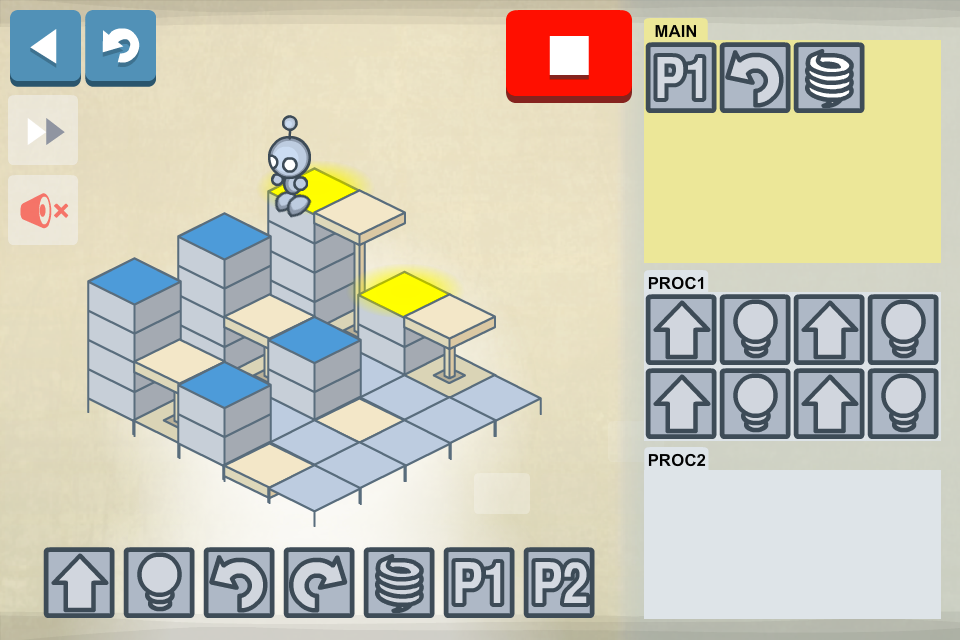
\includegraphics[scale=2.50]{LI1/li1g065/unnamed.jpg}
\caption{Tabuleiro do jogo \textit{LightBot}}
\end{figure}



\author{Fábio Baião A75662 João Coelho A74859} 
\date {\today}

\begin{document}

\maketitle

\tableofcontents

\section{Introdução ao Projeto}

% aqui será feita uma apresentação do projeto desenvolvido, com referências ao jogo que se pretende criar e restantes objetivos

\begin{itemize}
\item Um...
\item Dois...
\end{itemize}

\subsection{\textit{LighBot}}

% breve apresentação do jogo

\subsection{Objetivos do grupo}

% criar o nosso primeiro jogo é sempre marcante para estudantes de Eng Informática

\section{Tarefa 1}

% informação referente à primeira tarefa

\section{Tarefa 2}

% informação referente à segunda tarefa

\section{Tarefa 3}

% informação referente à terceira tarefa

\section{Conclusão}

\begin{enumerate}
    \item Um...
    \item Dois...
\end{enumerate}



\includegraphics[scale=0.50]{LI1/li1g065/Picture2.jpg}
\end{document}